\documentclass[]{article}
\usepackage{lmodern}
\usepackage{amssymb,amsmath}
\usepackage{ifxetex,ifluatex}
\usepackage{fixltx2e} % provides \textsubscript
\ifnum 0\ifxetex 1\fi\ifluatex 1\fi=0 % if pdftex
  \usepackage[T1]{fontenc}
  \usepackage[utf8]{inputenc}
\else % if luatex or xelatex
  \ifxetex
    \usepackage{mathspec}
  \else
    \usepackage{fontspec}
  \fi
  \defaultfontfeatures{Ligatures=TeX,Scale=MatchLowercase}
  \newcommand{\euro}{€}
\fi
% use upquote if available, for straight quotes in verbatim environments
\IfFileExists{upquote.sty}{\usepackage{upquote}}{}
% use microtype if available
\IfFileExists{microtype.sty}{%
\usepackage{microtype}
\UseMicrotypeSet[protrusion]{basicmath} % disable protrusion for tt fonts
}{}
\usepackage{hyperref}
\PassOptionsToPackage{usenames,dvipsnames}{color} % color is loaded by hyperref
\hypersetup{unicode=true,
            pdftitle={My YAML title},
            pdfborder={0 0 0},
            breaklinks=true}
\urlstyle{same}  % don't use monospace font for urls
\usepackage{graphicx,grffile}
\makeatletter
\def\maxwidth{\ifdim\Gin@nat@width>\linewidth\linewidth\else\Gin@nat@width\fi}
\def\maxheight{\ifdim\Gin@nat@height>\textheight\textheight\else\Gin@nat@height\fi}
\makeatother
% Scale images if necessary, so that they will not overflow the page
% margins by default, and it is still possible to overwrite the defaults
% using explicit options in \includegraphics[width, height, ...]{}
\setkeys{Gin}{width=\maxwidth,height=\maxheight,keepaspectratio}
\setlength{\parindent}{0pt}
\setlength{\parskip}{6pt plus 2pt minus 1pt}
\setlength{\emergencystretch}{3em}  % prevent overfull lines
\providecommand{\tightlist}{%
  \setlength{\itemsep}{0pt}\setlength{\parskip}{0pt}}
\setcounter{secnumdepth}{0}

\title{My YAML title}
\author{true}
\date{}
\newtheorem{theorem}{Teorema}
\AtBeginDocument{%
\renewcommand*\figurename{Figure}
\renewcommand*\tablename{Table}
}
\AtBeginDocument{%
\renewcommand*\listfigurename{List of Figures}
\renewcommand*\listtablename{List of Tables}
}
\usepackage{float}
\floatstyle{ruled}
\makeatletter
\@ifundefined{c@chapter}{\newfloat{codelisting}{h}{lop}}{\newfloat{codelisting}{h}{lop}[chapter]}
\makeatother
\floatname{codelisting}{Listing}
\newcommand*\listoflistings{\listof{codelisting}{List of Listings}}

% Redefines (sub)paragraphs to behave more like sections
\ifx\paragraph\undefined\else
\let\oldparagraph\paragraph
\renewcommand{\paragraph}[1]{\oldparagraph{#1}\mbox{}}
\fi
\ifx\subparagraph\undefined\else
\let\oldsubparagraph\subparagraph
\renewcommand{\subparagraph}[1]{\oldsubparagraph{#1}\mbox{}}
\fi

\begin{document}
\maketitle
\begin{abstract}
This is the abstract.

It consists of two paragraphs.
\end{abstract}

\section{Titlu}\label{titlu}

\subsection{Achiziția comprimată a semnalelor cu reprezentări
rare}\label{sec:stateart}

\subsubsection{Text}\label{text}

Am text \emph{italic} si \textbf{bold} si \emph{subliniat}.

\subsubsection{Ecuații}\label{sec:ecuatii}

O ecuație inline este \(p \geq 1\)

Aici am o ecuație:

\begin{equation}
 \|x\|_p = \left( \sum_i |x_i|^p \right) ^\frac{1}{p}
\label{eq:ec1}\end{equation}

si ma refer la ea ca ecuatia (eq.~\ref{eq:ec1}). E \textbf{obligatoriu}
ca ecuația să fie intr-un paragraf nou (separată cu linii goale inainte
și după),

O listă cu ecuații inline si separate:

\begin{enumerate}
\def\labelenumi{\arabic{enumi}.}
\item
  \(\|ax\| = |a| \cdot \|x\|\) (omogenitate)
\item
  Și încă una aici
\end{enumerate}

\begin{equation}\|x\| = 0 \iff x=0\label{eq:ec2}\end{equation}

\begin{enumerate}
\def\labelenumi{\arabic{enumi}.}
\tightlist
\item
  \(\|x + y\| \leq \|x\| + \|y\|\) (inegalitatea triunghiului)
\end{enumerate}

si o citez pe ultima ca (eq.~\ref{eq:ec2}).

Din păcate, pentru ca trebuie să pun ecuația într-un paragraf nou,
\textbf{se întrerupe numerotarea}!!

Și încă o ecuație cu cuvinte în interior (\emph{unde}) și cazuri (): \[
 \|x\|_0 = \sum_{i}^{} c_i, \textrm{ unde } c_i = \begin{cases} 1 , x_i \neq 0 \\ 0 , x_i = 0 \end{cases} 
\]

\subsubsection{Figuri}\label{figuri}

În Figura 1 sunt înfățișate sferele \(\ell_p\) într-un spațiu
bidimensional, adică punctele care au aceeași valoare a normei
\(\ell_p\) (aici, egală cu 1), pentru diverse valori ale lui \(p\).
Pentru \(p = 0\), domeniul cuprinde doar cele două axe (exceptând
punctul 0). Se observă că valori mici ale lui \(p\) implică puncte
situate în apropierea celor două axe, funcționând astfel ca niște
aproximații ale normei \(\ell_0\).

\begin{figure}[htbp]
\centering
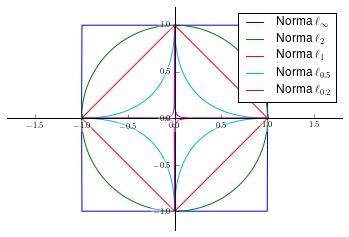
\includegraphics{lpnorms.png}
\caption{Figura 1 - Punctele dintr-un plan care au norma \(\ell_p\)
egală cu 1}
\end{figure}

\subsubsection{Teoreme, definiții,
citari}\label{teoreme-definiux21bii-citari}

Definiție ca text:

\textbf{Definiţie.} {[}1{]}: Fie matricea
\(A \in \mathbb{R}^{m \times n}\). \emph{Spark}-ul matricii \(A\), notat
\(\sigma\), reprezintă numărul minim de coloane ale lui \(A\) care sunt
liniar independente.

Următoarea este o teoremă cu demonstrație, ca text:

\begin{theorem}

{[}1{]}: Fie \(\gamma\) un vector rar cu \(\|\gamma\|_0 = k\),
achiziţionat cu o matrice \(A\) ca în (eq.~\ref{eq:ec1}). Fie \(\sigma\)
\emph{spark}-ul matricii \(A\). Dacă \(k < \sigma / 2\), atunci
\(\gamma\) este soluţie unică a problemei de optimizare
(eq.~\ref{eq:ec2}).

\end{theorem}

\emph{Demonstraţie.} Demonstraţia rezultă imediat: dacă
(eq.~\ref{eq:ec1}) ar admite o soluţie diferită, cu raritatea
\(k' \leq k\), atunci diferenţa celor două soluţii ar produce un vector
de raritate \((k'+k) < \sigma\) care aparţine spaţiului nul al matricii
\(A\). Acest lucru înseamnă un set de coloane liniar independente ale
lui \(A\) în număr mai mic decât \emph{spark}-ul matricii, ceea ce
contrazice definiţia acestuia.

Din păcate, calcularea \emph{spark}-ului unei matrici este o problemă de
complexitate combinatorică, şi deci \emph{NP-hard}, ceea ce limitează
aplicabilitatea practică a teoremei.

Aici mai vine o teorema, ca sa verific daca numerele sunt puse bine:

\begin{theorem}

{[}1{]}: Alta teorema domnule.

\end{theorem}

\emph{Demonstraţie.} Demonstraţia rezultă imediat, domnule.

\subsubsection{Algoritmi}\label{algoritmi}

\textbf{Algoritmul Orthogonal Matching Pursuit (OMP)}

\emph{Fenced clode block}:

\begin{verbatim}
   1. $r^{(0)} \leftarrow y$
   2. $\gamma_i \leftarrow 0, \forall i$
   3. repetă:  
       3.1.    Găsește $a_m \in A$ cu coeficientul de corelația maxim $\left\langle r^{(k)}, a_m \right\rangle$  
       3.2.    Adaugă $m$ la setul indicilor atomilor selectați, $T \leftarrow T \cup \{m\}$  
       3.3.    Proiectează $x$ pe subspațiul atomilor $a_{\{T\}}$, obținând vectorul coeficienților de la pasul $k$: $\gamma_{\{T\}}^{(k+1)} = a_{\{T\}}^{\dagger} x$  
       3.4.    Actualizează reziduul: $r^{(k+1)} \leftarrow x - A \cdot \gamma^{(k+1)}$
   4. până la un criteriu de oprire (de ex. $\|r^{(k)}\|_2 \le \epsilon$, sau număr fixat de iterații}  
\end{verbatim}

sau \emph{clode block} normal (cu 4 spații):

\begin{verbatim}
1. $r^{(0)} \leftarrow y$
2. $\gamma_i \leftarrow 0, \forall i$
3. repetă:  
    3.1.    Găsește $a_m \in A$ cu coeficientul de corelația maxim $\left\langle r^{(k)}, a_m \right\rangle$  
    3.2.    Adaugă $m$ la setul indicilor atomilor selectați, $T \leftarrow T \cup \{m\}$  
    3.3.    Proiectează $x$ pe subspațiul atomilor $a_{\{T\}}$, obținând vectorul coeficienților de la pasul $k$: $\gamma_{\{T\}}^{(k+1)} = a_{\{T\}}^{\dagger} x$  
    3.4.    Actualizează reziduul: $r^{(k+1)} \leftarrow x - A \cdot \gamma^{(k+1)}$
4. până la un criteriu de oprire (de ex. $\|r^{(k)}\|_2 \le \epsilon$, sau număr fixat de iterații}  
\end{verbatim}

Din păcate, în \emph{code blocks} nu se parsează ecuațiile Latex.
Singura soluție este să le scriu ca liste obișnuite (de ex. cu 3
spații):

\begin{enumerate}
\def\labelenumi{\arabic{enumi}.}
\tightlist
\item
  \(r^{(0)} \leftarrow y\)
\item
  \(\gamma_i \leftarrow 0, \forall i\)
\item
  repetă:\\
   3.1. Găsește \(a_m \in A\) cu coeficientul de corelația maxim
  \(\left\langle r^{(k)}, a_m \right\rangle\)\\
   3.2. Adaugă \(m\) la setul indicilor atomilor selectați,
  \(T \leftarrow T \cup \{m\}\)\\
   3.3. Proiectează \(x\) pe subspațiul atomilor \(a_{\{T\}}\), obținând
  vectorul coeficienților de la pasul \(k\):
  \(\gamma_{\{T\}}^{(k+1)} = a_{\{T\}}^{\dagger} x\)\\
   3.4. Actualizează reziduul:
  \(r^{(k+1)} \leftarrow x - A \cdot \gamma^{(k+1)}\)
\item
  până la un criteriu de oprire (de ex. \(\|r^{(k)}\|_2 \le \epsilon\),
  sau număr fixat de iterații\}
\end{enumerate}

\subsubsection{Tabele}\label{tabele}

TODO

\hypertarget{refs}{}
\hypertarget{ref-OptimSpReprDonoho2003}{}
{[}1{]} D. L. Donoho and M. Elad, ``Optimally sparse representation in
general (nonorthogonal) dictionaries via l1 minimization,''
\emph{Proceedings of the National Academy of Sciences}, vol. 100, no. 5,
pp. 2197--2202, 2003.

\end{document}
